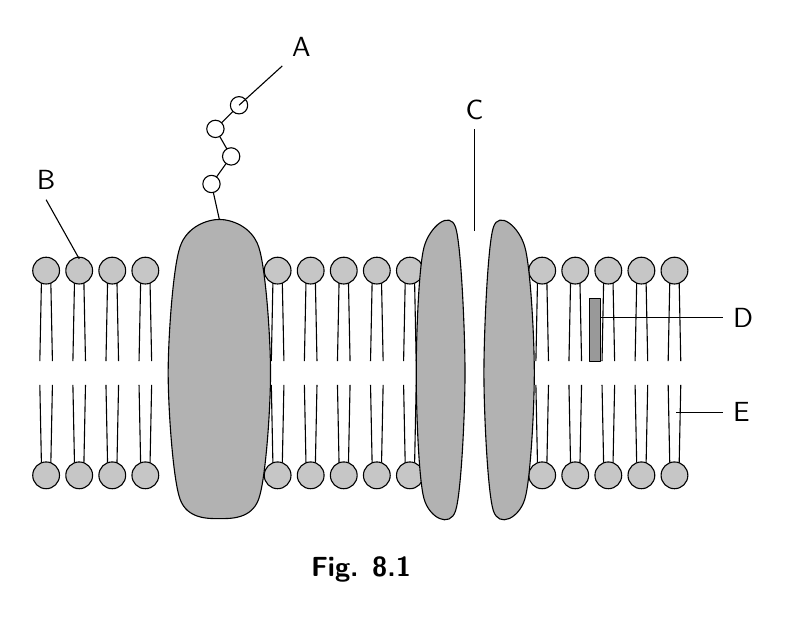
\begin{tikzpicture}[font=\sffamily, line join=round]
  % phospholipid bilayer, leaving gaps for the proteins
  \foreach \i in {0,...,19} {
    \pgfmathsetmacro{\x}{0.3+\i*0.42}
    \pgfmathparse{(\x>1.9 && \x<3.1) || (\x>5.0 && \x<6.5) ? 1 : 0}
    \ifnum\pgfmathresult=0
      \draw[thin] (\x-0.06,2.44)--(\x-0.08,1.45) (\x+0.06,2.44)--(\x+0.08,1.45);
      \draw[thin] (\x-0.06,0.16)--(\x-0.08,1.15) (\x+0.06,0.16)--(\x+0.08,1.15);
      \draw[thin, fill=gray!45] (\x,2.6) circle (0.17) (\x,0) circle (0.17);
    \fi
  }
  % proteins
  \draw[fill=gray!60] plot[smooth cycle] coordinates {(2.0,-0.3) (1.85,1.3) (2.0,2.9) (2.5,3.25) (3.0,2.9) (3.15,1.3) (3.0,-0.3) (2.5,-0.55)};
  \draw[fill=gray!60] plot[smooth cycle] coordinates {(5.1,-0.3) (5.0,1.3) (5.1,2.9) (5.5,3.15) (5.62,1.3) (5.5,-0.45)};
  \draw[fill=gray!60] plot[smooth cycle] coordinates {(6.38,-0.3) (6.5,1.3) (6.38,2.9) (5.98,3.15) (5.86,1.3) (5.98,-0.45)};
  % carbohydrate chain on the glycoprotein
  \draw (2.5,3.25)--(2.4,3.7)--(2.65,4.05)--(2.45,4.4)--(2.75,4.7);
  \foreach \p in {(2.4,3.7),(2.65,4.05),(2.45,4.4),(2.75,4.7)} \draw[fill=white] \p circle (0.11);
  % cholesterol
  \draw[fill=gray!80] (7.2,1.45) rectangle (7.34,2.25);
  % labels
  \draw (2.75,4.7)--(3.3,5.2) node[above right] {A};
  \draw (0.72,2.75)--(0.3,3.5) node[above] {B};
  \draw (5.74,3.1)--(5.74,4.4) node[above] {C};
  \draw (7.34,2.0)--(8.9,2.0) node[right] {D};
  \draw (8.3,0.8)--(8.9,0.8) node[right] {E};
  \node[font=\sffamily\bfseries] at (4.3,-1.2) {Fig. 8.1};
\end{tikzpicture}
